\section{Internet Traffic Censorship}
Censorship of Internet traffic occurs in a variety of forms all over the world. The most aggressive censorship takes place in countries where citizens' access to the Internet is very limited to begin with (e.g., North Korea and Cuba). Verkamp and Gupta \cite{Verkamp2012} conducted experiments to infer the mechanics of various countries' approaches to Internet censorship and also provided a set of independent sources ranking countries based on the severity of their censorship. 

\begin{figure}[h]
\centering
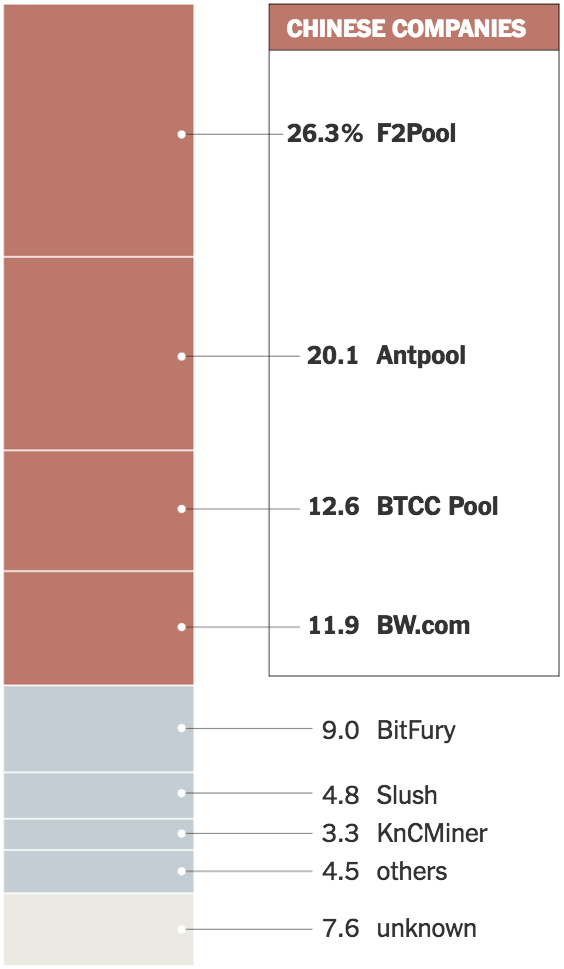
\includegraphics[height=250pt]{Images/NYT-Bitcoin-China.png}
\caption{From \cite{Popper2016}: the shares of mined Bitcoin blocks from May 24 to June 24, 2016 by mining pool.}
\label{fig:BTCPools}
\end{figure}

Across our research, four countries were repeatedly identified as the most severe Internet censors: North Korea, Cuba, Iran, and China. Of these, China is the most interesting case for our purposes for two reasons: (1) its Internet-connected population far surpasses the others' and (2) it is a hotbed of Bitcoin mining activity, with Chinese-run mining pools accounting for an estimated 70\% of all Bitcoin mining power as of June 2016 (Figure~\ref{fig:BTCPools}). As a collection, China's censorship measures are colloquially referred to as The Great Firewall of China (GFW).

\subsection{The Great Firewall of China}
Existing research describes the primary techniques used by the GFW to censor Internet traffic \cite{GFWStanford}.

\begin{itemize}
\item \textit{IP address filtering}:
For well-known sites that China has decided to ban, the GFW will drop all packets associated with a particular IP address. This assures that the GFW?s reach extends to all content produced by a host's IP, rather than just a few specified domains.

\item \textit{DNS misdirection (hijacking)}:
When requesting a blocked host name, there are cases in which the DNS servers under the GFW will return a different IP address than the one that corresponds to the domain name requested. The Chinese government can effectively replace the content with material that is more favorable to their interests.

\item \textit{Keyword filtering}:
If a banned keyword appears in a URL, after a completed TCP handshake, the GFW will send reset packets to both the source and destination, blocking access to the requested content. Even if a keyword is not explicitly in the URL but appears within the HTML response, the content is also denied. In this particular instance, pages often begin to display but are then truncated after the discovery of a keyword.
\end{itemize}

\subsubsection{Impact on Bitcoin}
These techniques censor web-browsing traffic, but will not interfere with Bitcoin traffic. However, the GFW does introduce an overall delay for all traffic, and so due to this and normal Bitcoin propagation delays, Chinese miners will hear about blocks mined outside of China later than ones within the country, causing a communication barrier. This also creates an unfair disadvantage to those outside of China since China has majority hash power. This can constrain Bitcoin itself in some ways such as during the controversy surrounding a proposed block size increase. If the size were to increase, Chinese miners would be subject to further delays, potentially jeopardizing profits.




\cite{Xu2011}